%%%%%%%%%%%%%%%%%%%%%%%%%%%%%%%%%%%%%%%%%
% Short Sectioned Assignment LaTeX Template Version 1.0 (5/5/12)
% This template has been downloaded from: http://www.LaTeXTemplates.com
% Original author:  Frits Wenneker (http://www.howtotex.com)
% License: CC BY-NC-SA 3.0 (http://creativecommons.org/licenses/by-nc-sa/3.0/)
%%%%%%%%%%%%%%%%%%%%%%%%%%%%%%%%%%%%%%%%%

%----------------------------------------------------------------------------------------
%	PACKAGES AND OTHER DOCUMENT CONFIGURATIONS
%----------------------------------------------------------------------------------------

\documentclass[paper=a4, fontsize=11pt]{scrartcl} % A4 paper and 11pt font size

% ---- Entrada y salida de texto -----

\usepackage[T1]{fontenc} % Use 8-bit encoding that has 256 glyphs
\usepackage[utf8]{inputenc}
%\usepackage{fourier} % Use the Adobe Utopia font for the document - comment this line to return to the LaTeX default

% ---- Idioma --------

\usepackage[spanish, es-tabla]{babel} % Selecciona el español para palabras introducidas automáticamente, p.ej. "septiembre" en la fecha y especifica que se use la palabra Tabla en vez de Cuadro

% ---- Otros paquetes ----

\usepackage{url} % ,href} %para incluir URLs e hipervínculos dentro del texto (aunque hay que instalar href)
\usepackage{amsmath,amsfonts,amsthm} % Math packages
%\usepackage{graphics,graphicx, floatrow} %para incluir imágenes y notas en las imágenes
\usepackage{graphics,graphicx, float} %para incluir imágenes y colocarlas

% Para hacer tablas comlejas
%\usepackage{multirow}
%\usepackage{threeparttable}

%\usepackage{sectsty} % Allows customizing section commands
%\allsectionsfont{\centering \normalfont\scshape} % Make all sections centered, the default font and small caps

\usepackage{fancyhdr} % Custom headers and footers
\pagestyle{fancyplain} % Makes all pages in the document conform to the custom headers and footers
\fancyhead{} % No page header - if you want one, create it in the same way as the footers below
\fancyfoot[L]{} % Empty left footer
\fancyfoot[C]{} % Empty center footer
\fancyfoot[R]{\thepage} % Page numbering for right footer
\renewcommand{\headrulewidth}{0pt} % Remove header underlines
\renewcommand{\footrulewidth}{0pt} % Remove footer underlines
\setlength{\headheight}{13.6pt} % Customize the height of the header

\numberwithin{equation}{section} % Number equations within sections (i.e. 1.1, 1.2, 2.1, 2.2 instead of 1, 2, 3, 4)
\numberwithin{figure}{section} % Number figures within sections (i.e. 1.1, 1.2, 2.1, 2.2 instead of 1, 2, 3, 4)
\numberwithin{table}{section} % Number tables within sections (i.e. 1.1, 1.2, 2.1, 2.2 instead of 1, 2, 3, 4)

\setlength\parindent{0pt} % Removes all indentation from paragraphs - comment this line for an assignment with lots of text

\newcommand{\horrule}[1]{\rule{\linewidth}{#1}} % Create horizontal rule command with 1 argument of height

%\documentclass{report}
\usepackage{blindtext}
\usepackage{hyperref}
\usepackage{listings}
\usepackage{graphicx}
\graphicspath{ {images/} }

\title{	
\normalfont \normalsize 
\textsc{\textbf{Sistemas Gráficos (2022-2023)} \\ Grado en Ingeniería Informática \\ Universidad de Granada} \\ [25pt] % Your university, school and/or department name(s)
\horrule{0.5pt} \\[0.4cm] % Thin top horizontal rule
\huge Documentación Práctica 2 - Scape Room \\ % The assignment title
\horrule{2pt} \\[0.5cm] % Thick bottom horizontal rule
}

\author{Francisco Javier Gallardo Molina} % Nombre y apellidos

\date{\normalsize\today} % Incluye la fecha actual

\renewcommand{\footrulewidth}{0.4pt}
\lfoot[]{Francisco Javier Gallardo Molina}
\rfoot[]{\thepage}

\begin{document}

\maketitle

\newpage

\horrule{1pt}
\tableofcontents

\newpage

\section{Descripción de la aplicación}

La práctica trata de realizar un Scape Room hecho con JavaScript junto con three.js y WebGL. Para ello es necesario también un servidor web como lo puede ser Apache. En mi caso, usé una imagen de Docker que contenía el servidor de Apache por defecto para agilizar y facilitar la instalación del entorno de trabajo (Dockerfile adjuntado en el archivo zip). En la concreción de la aplicación, se aprobó la siguiente explicación:\\

\textit{El Scape room trata de robar una figura oculta de una colección privada y hay que realizar distintas acciones para descubrir el escondite de dicha figura. La habitación será en forma de L y contendrá una serie de muebles con los que se interactuarán. Primero habrá que realizar un pequeño puzle en una mesa que hará que el cuadro descubra detrás un trofeo (el cuadro es el objeto articulado). Segundo, el trofeo se deberá de colocar encima del pedestal. Eso activará otra cosa aún por definir y con otro par de cosas sin definir (puede ser que se incluyan en una segunda sala) con las que se descubrirá el escondrijo de la figura en la puerta de salida. También habrá un reloj que será la figura que tenga el continuo movimiento de las manecillas. En la imagen adjuntada a continuación se ven con más detalle la forma de la sala y los elementos que contiene de momento (se ha dibujado la sala desde dos ángulos distintos)} \ref{fig:definicion}

\begin{figure}[H]
  \centering
  \includegraphics[scale=0.07,angle=-90,origin=c]{imagen_definicion}
  \caption{Definición inicial del scape room}
  \label{fig:definicion}
\end{figure}

Cabe destacar que han habido ciertos cambios en la realización del Scape Room. El puzle encima de la mesa fue cambiado por un puzle de luces en la pared, que en lugar de descubrir un trofeo detrás de un cuadro, permitía el acceso a un panel numérico. La colocación del trofeo en el pedestal se ha mantenido. La segunda sala fue incluida finalmente(una sala interior). El reloj también se ha mantenido.

\section{Diseño de la aplicación}

\subsection{Detalles del diseño}
\subsubsection{Modelado de objetos}
Para el modelador de objetos, he usado distintas metodologías, en conjunto o por separado. Se han usado técnicas de revolución, extrusión, barrido, CSG y carga de objetos OBJ:

\begin{enumerate}
\item Revolución: Trofeo
\item Extrusión: Figura Rara 1 
\item Barrido: Figura Rara 2
\item CSG: Pedestal, Trofeo, Habitación, Cuadro, Taza
\item Objeto OBJ: \href{https://free3d.com/3d-model/cinema4d-table-66762.html}{Mesa}
\end{enumerate}

En las imágenes \ref{fig:figuras} y \ref{fig:mesa} se pueden ver ejemplos de estos modelados.

\begin{figure}[H]
  \centering
  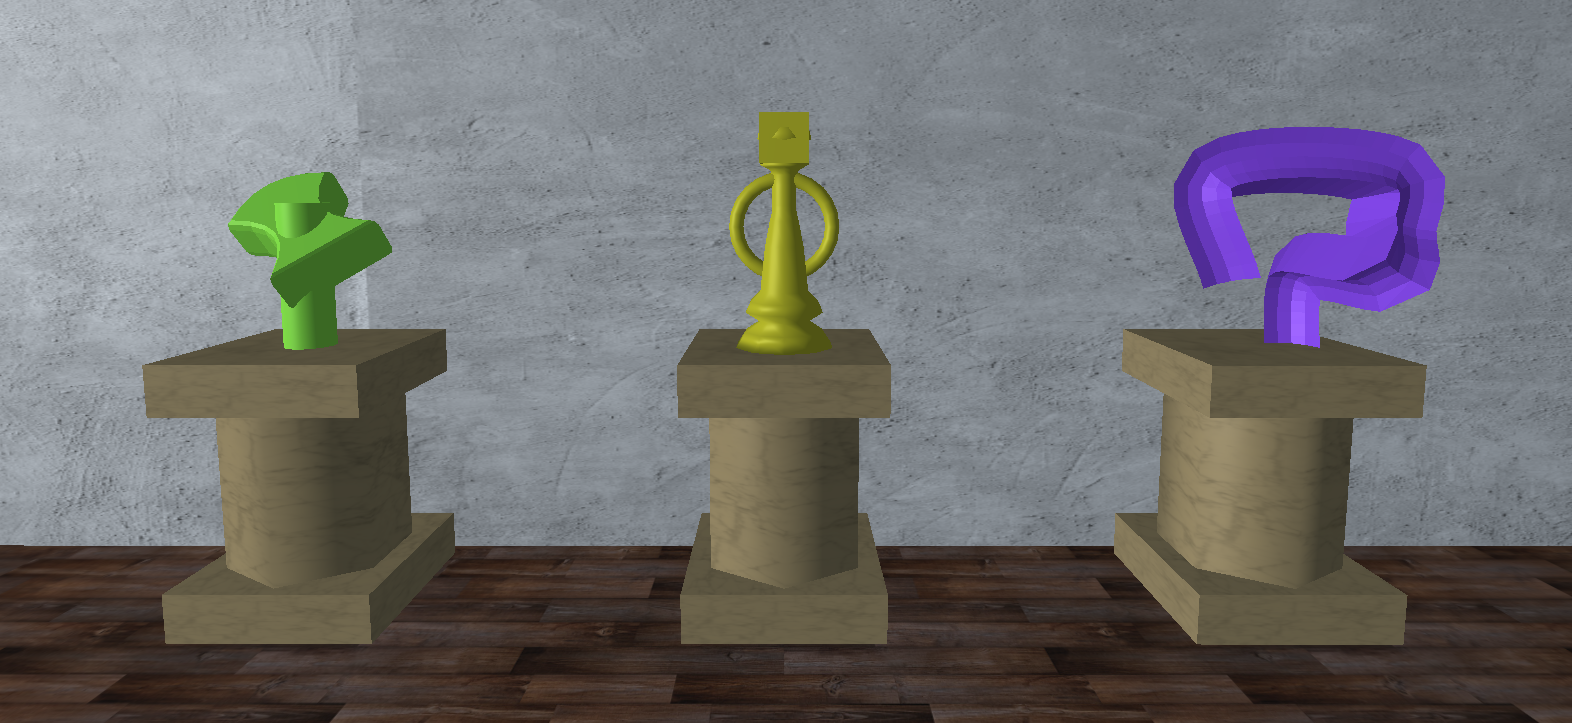
\includegraphics[scale=0.3]{piezas}
  \caption{Ejemplo de modelado 1}
  \label{fig:figuras}
\end{figure}

\begin{figure}[H]
  \centering
  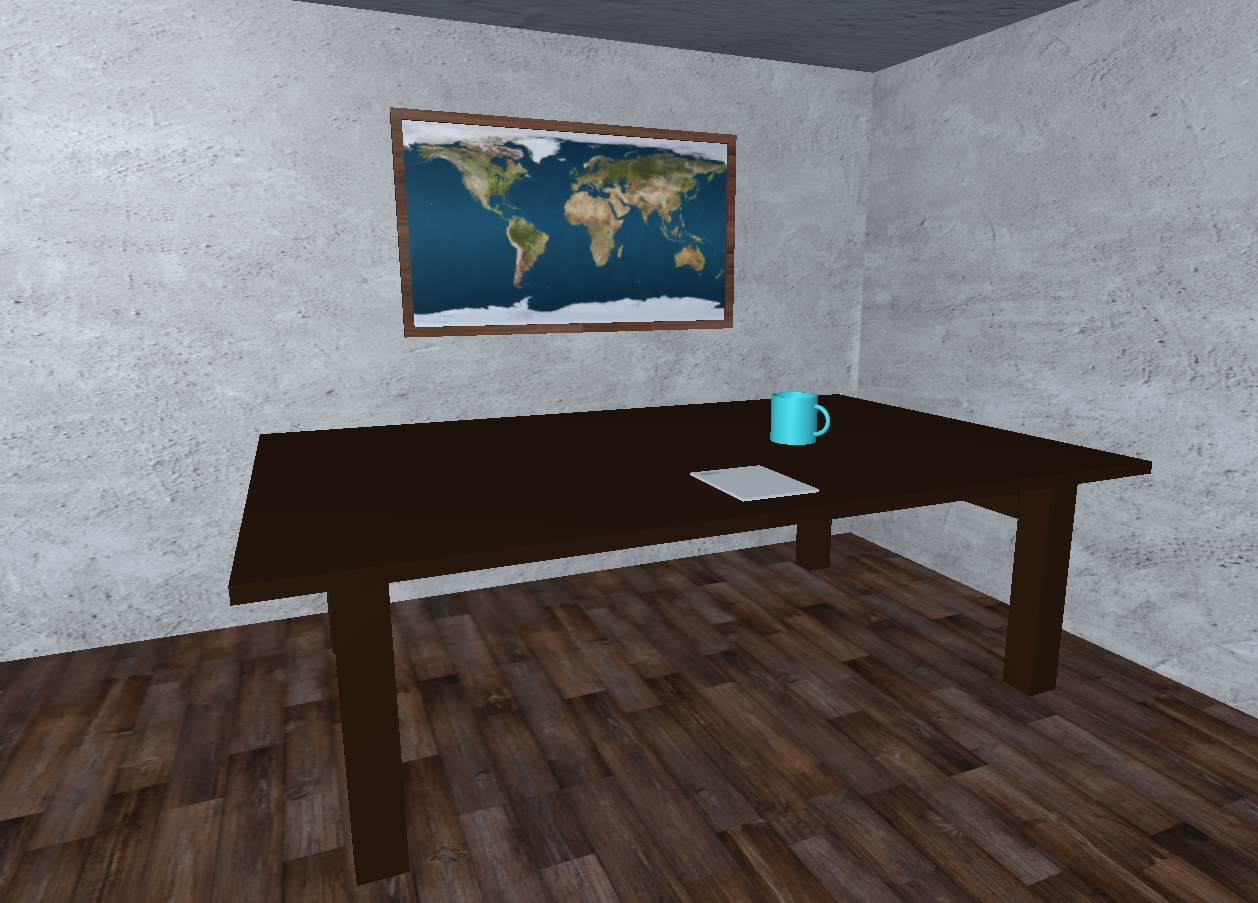
\includegraphics[scale=0.25]{mesa}
  \caption{Ejemplo de modelado 2}
  \label{fig:mesa}
\end{figure}

\subsubsection{Materiales}
Se han usado materiales tanto \textit{MeshPhongMaterial} como \textit{MeshLambertMaterial} para el uso de texturas y simulación de luces en objetos, así como transparencia o colores simples.

\begin{figure}[H]
  \centering
  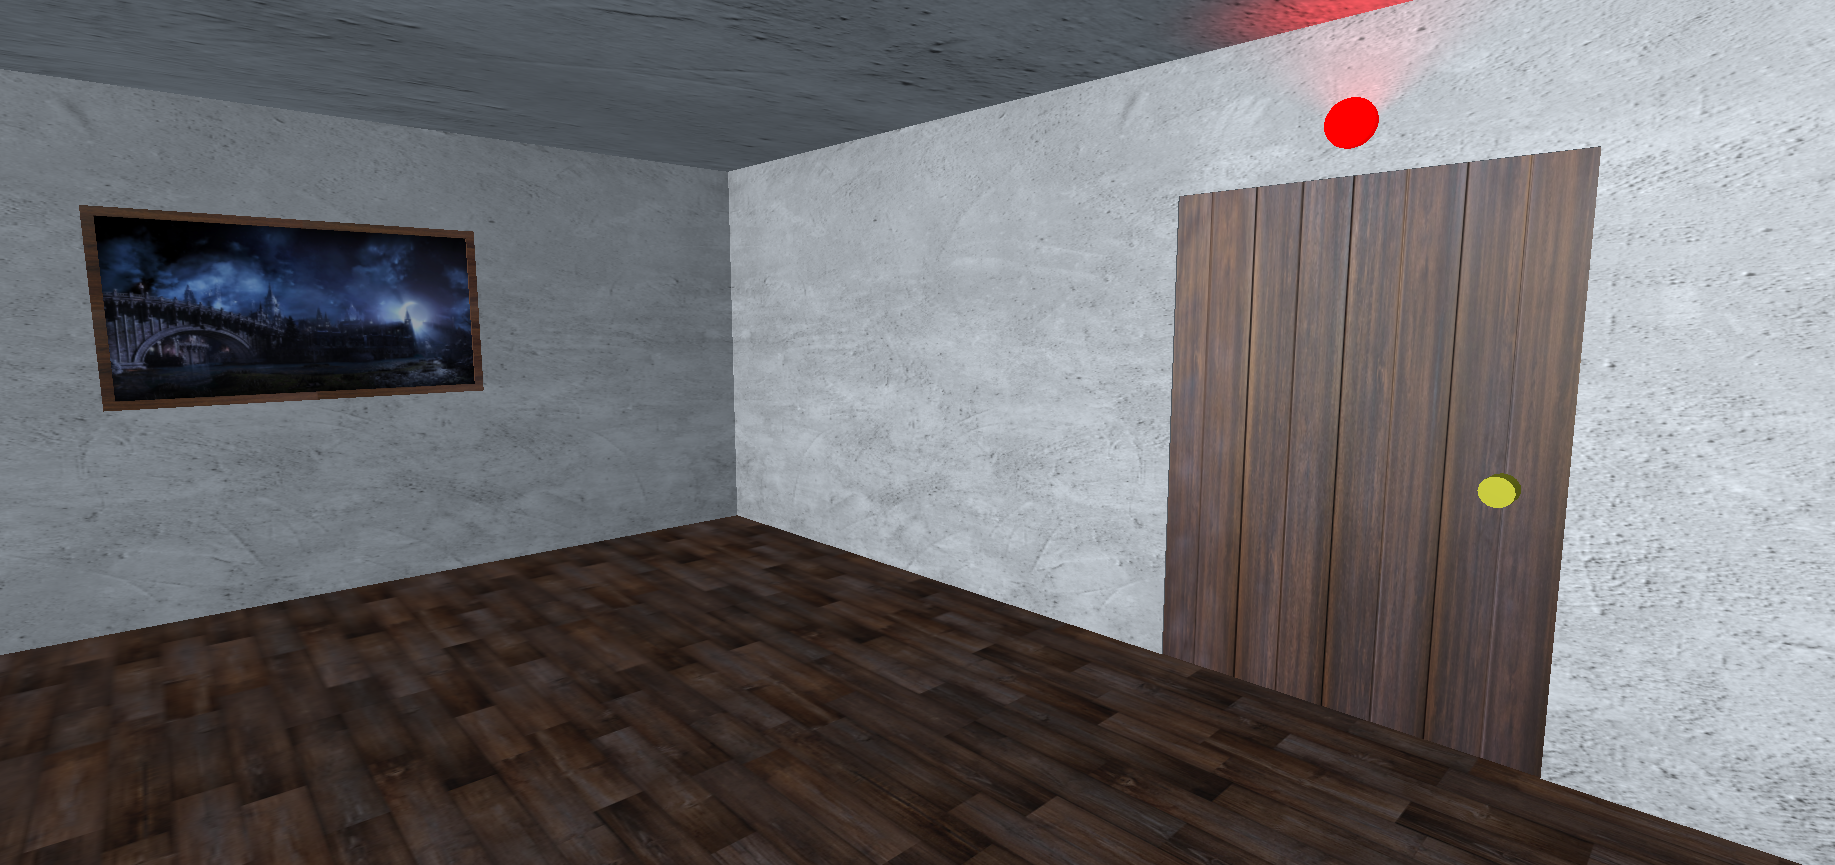
\includegraphics[scale=0.2]{habitacion}
  \caption{Diferentes materiales de la habitación}
  \label{fig:materiales}
\end{figure}

En la imagen \ref{fig:materiales} se aprecia en las paredes, suelo, puerta y cuadro que están hechos con una textura. El pomo tiene un color base amarillo y la luz roja es un material con componente \textit{emissive} para indicar que es una luz encendida.
\subsubsection{Luces}
Se ha desarrollado una clase nueva adicional que incluyen luces \textit{SpotLight}, un objeto \textit{Object3D} como target y una esfera como representación de lámpara para facilitar su creación y tambiém para simplificar y modularizar el código. También se ha usado \textit{PointLight} como lámpara normal de la sala y \textit{AmbientLight} para que no haya oscuridad.

\begin{figure}[H]
  \centering
  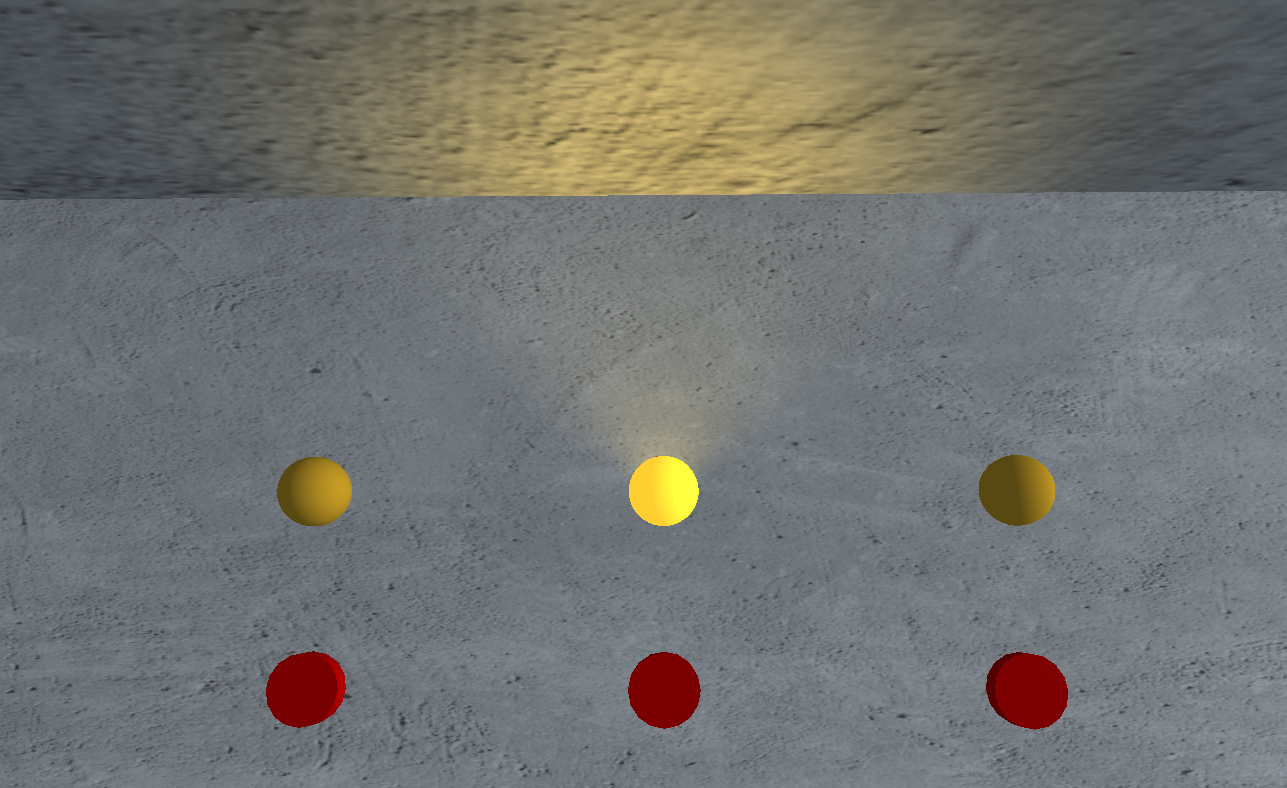
\includegraphics[scale=0.2]{luces}
  \caption{Luces encendidas y apagadas}
  \label{fig:luces}
\end{figure}

\subsubsection{Cámara}
Se han empleado tres cámaras distintas. La primera cámara es la personal, la cámara que simula la primera persona. La segunda cámara \ref{fig:camara} es la que se activa cuando pinchamos el panel numérico para que vea en primera plana y la última cámara que apunta a la puerta de salida encargada de la animación final.

\begin{figure}[H]
  \centering
  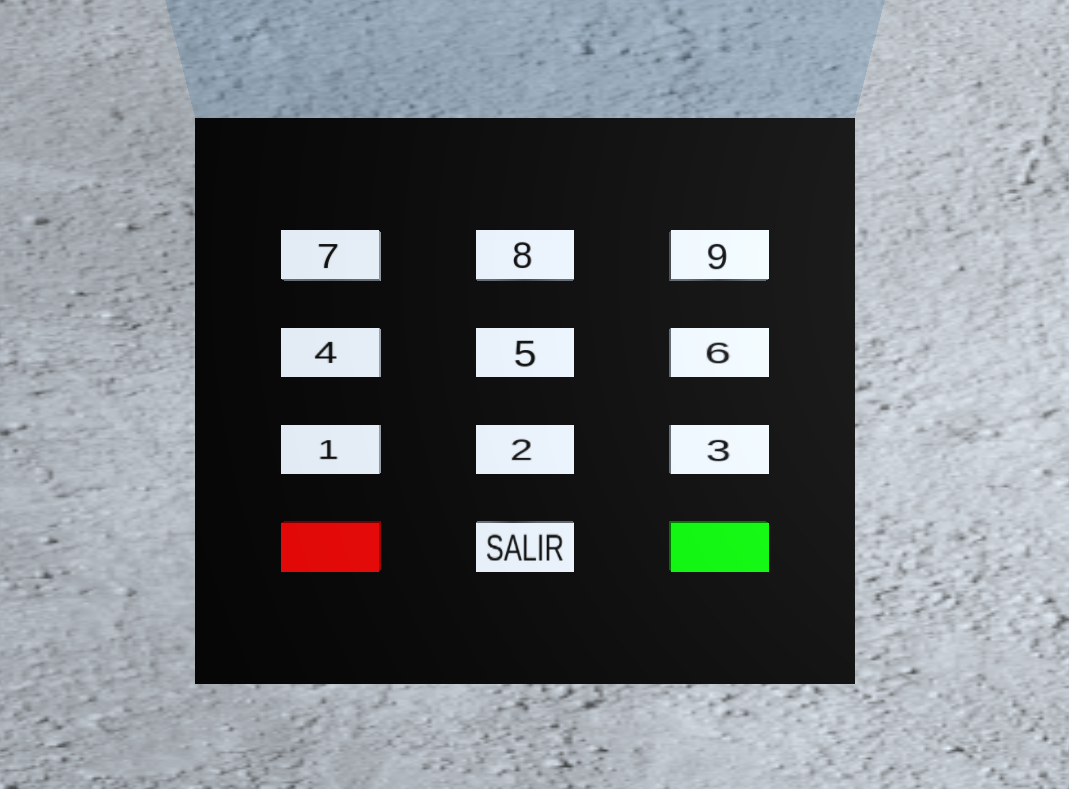
\includegraphics[scale=0.2]{camara}
  \caption{Cámara del panel numérico}
  \label{fig:camara}
\end{figure}

\subsection{Diagrama de clases}

El diagrama de clases \ref{fig:diagrama} se compone del objeto \textit{MyScene} que hereda de \textit{THREE.Scene}, en donde se incluyen el resto de objetos que componen toda la habitación. Dichos objetos heredan todos de la clase \textit{THREE.Object3D}.

\begin{figure}[H]
  \centering
  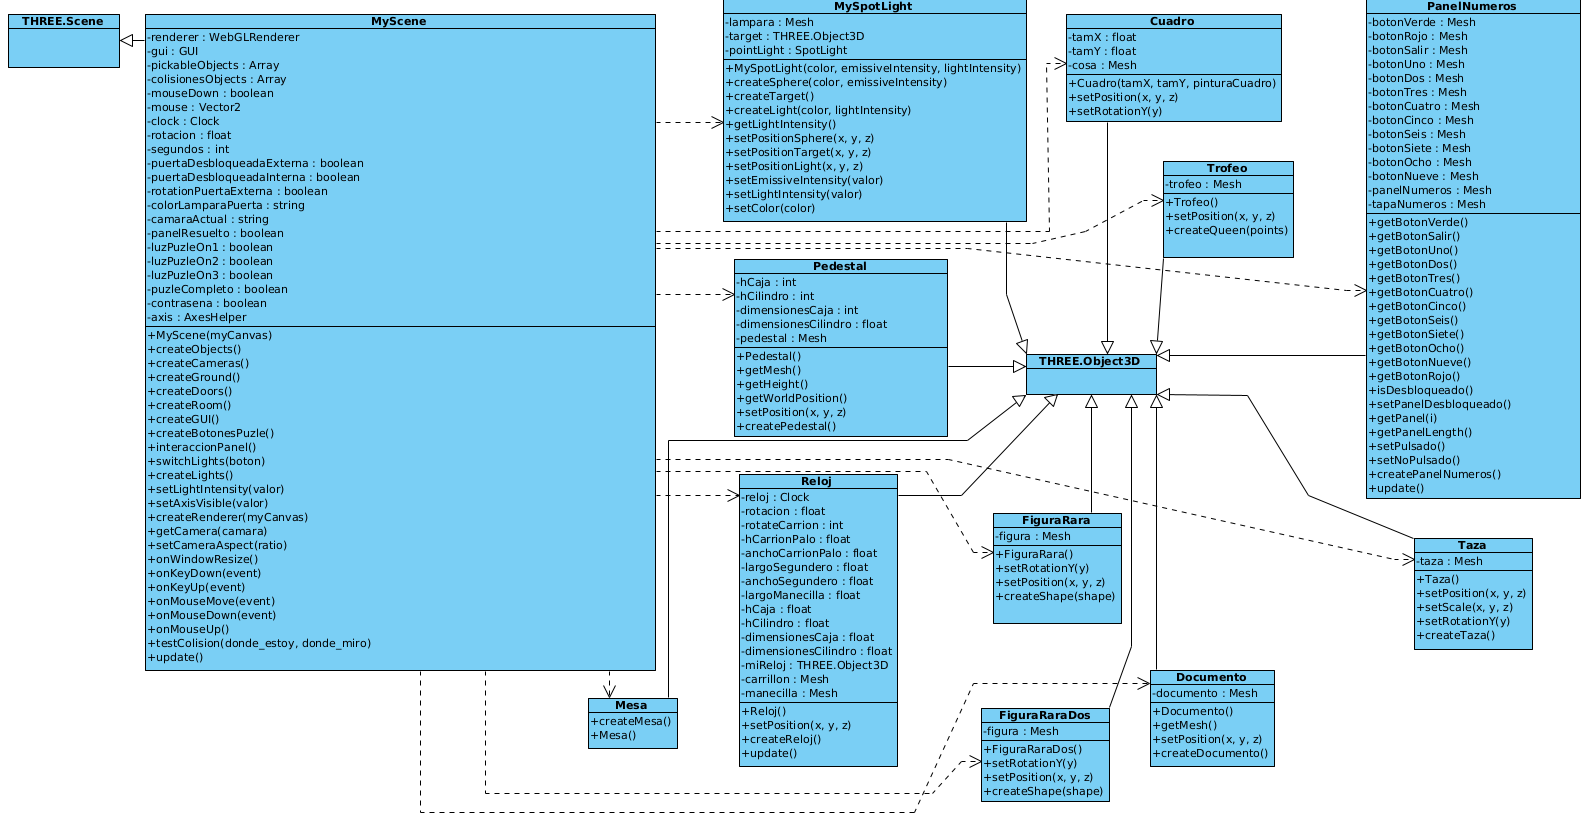
\includegraphics[scale=0.3]{diagrama}
  \caption{Diagrama de clases}
  \label{fig:diagrama}
\end{figure}

Se ha adjuntado la imagen del diagrama de clases por si se desea leer con mayor facilidad y detenimiento.

\newpage

\subsection{Modelo jerárquico}
El modelo jerárquico \ref{fig:jerarquico} se trata de un reloj cuyo carrillón y segundero están en constante movimiento. Cada golpe que da el carrillón a cada lado hace que avance un segundo la manecilla del segundero.

\begin{figure}[H]
  \centering
  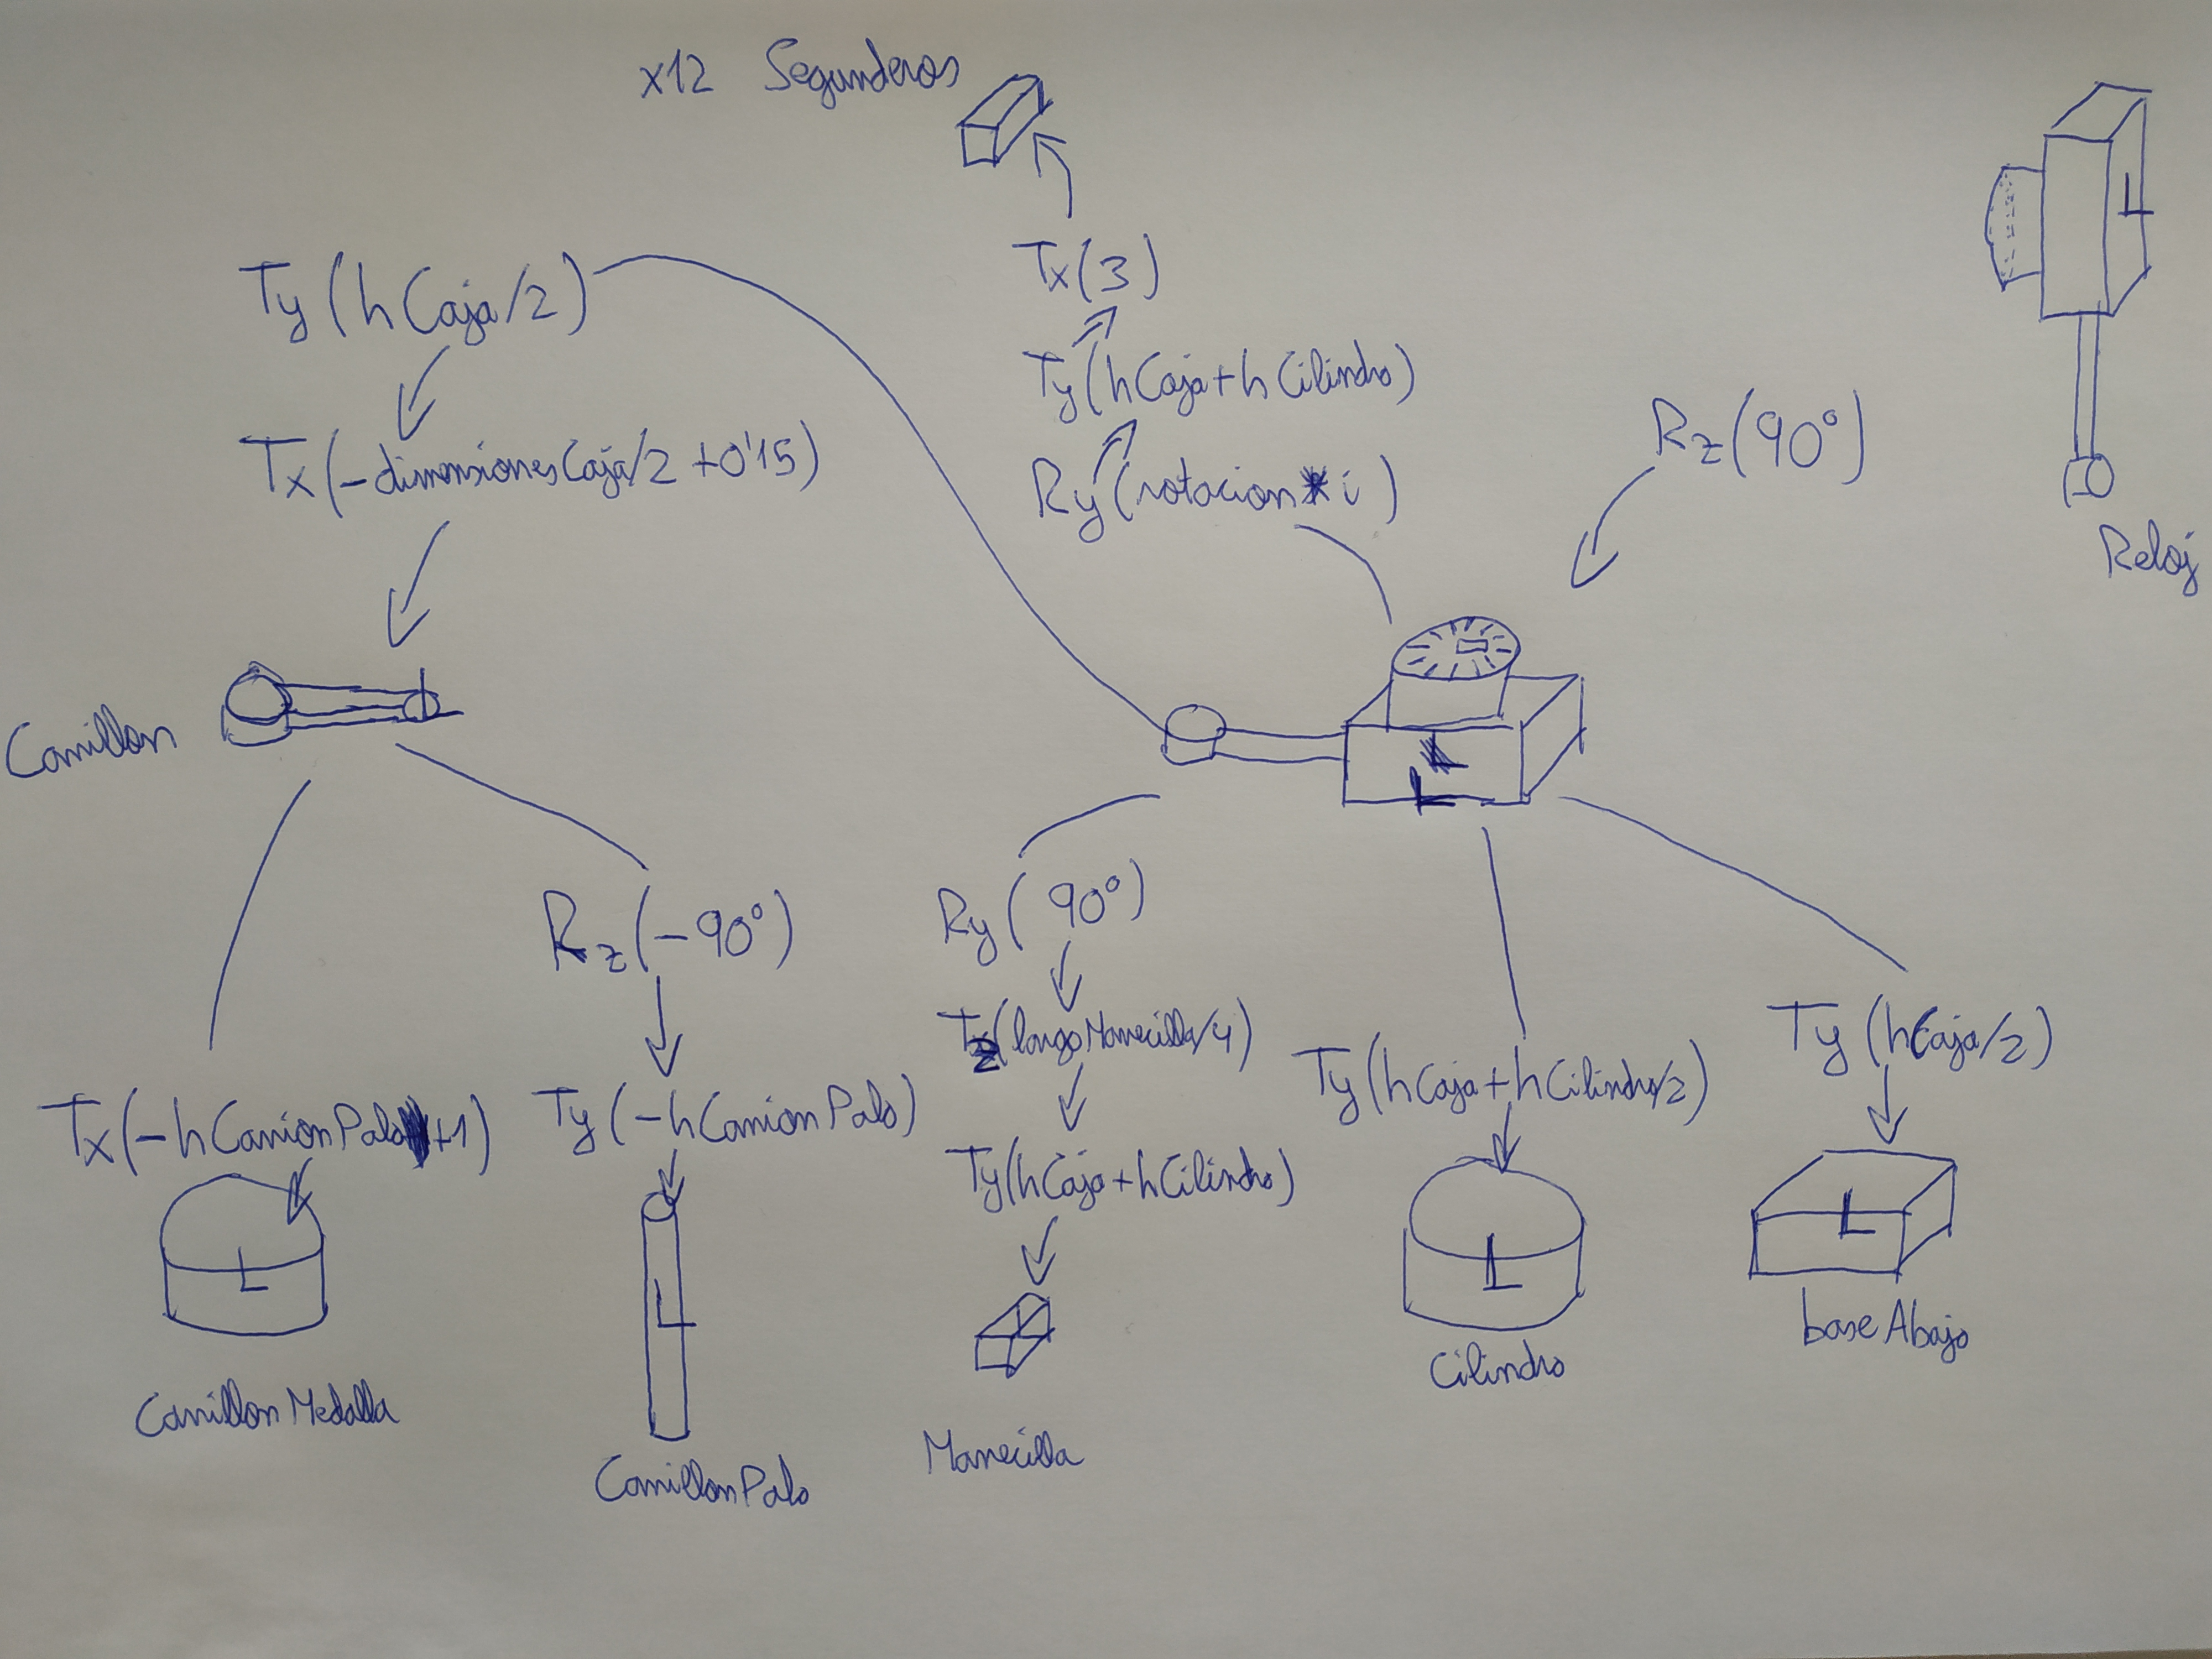
\includegraphics[scale=0.09]{modelo-jerarquico}
  \caption{Modelo jerárquico}
  \label{fig:jerarquico}
\end{figure}

El objeto en cuestión dentro de la escena es el siguiente:

\begin{figure}[H]
  \centering
  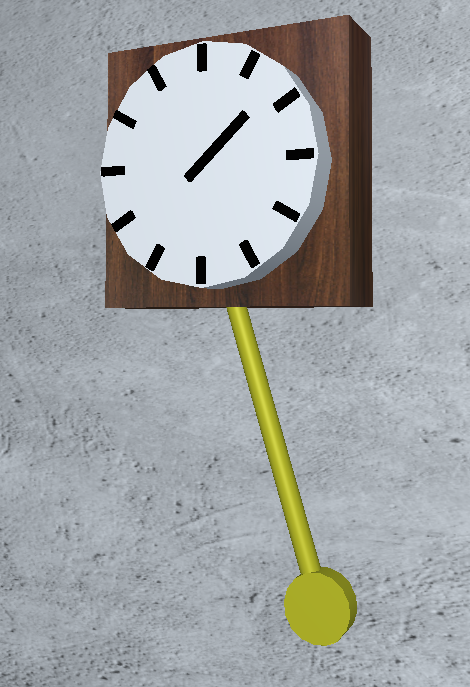
\includegraphics[scale=0.2]{reloj2}
  \caption{Reloj en la escena}
  \label{fig:reloj}
\end{figure}

\subsection{Descripción de algoritmos más importantes}

\textbf{interaccionPanel} - 
Este método es el encargado de la interacción con el panel numérico donde se introduce el código numérico. Detecta cada tecla, que hace lo que mueva y simule su pulsación, además de añadir números a la contraseña, borrarlos o comprobar si se ha introducido bien la clave numérica.\\\\
\textbf{switchLights} - 
Este método se encarga de encender o apagar las luces del puzle cuando se pulsan los botones e indicar cuáles son las luces que están encendidas o apagadas.\\\\
\textbf{onMouseDown} - 
Este método es el responsable de la interacción del cursor con los objetos de la escena. Se encarga de la propia interacción con el panel numérico, con la pulsación de los botones del puzle de luces, de abrir la puerta al terminar o de leer el documento de la mesa.\\\\
\textbf{onMouseMove} - 
Este método se encarga de la detección y movimiento de los objetos que son seleccionables. Concretamente, del objeto trofeo. Detecta cuando se ha clicado encima y cuando se está moviendo por la escena. También detecta si toca el pedestal al que tiene que ir para colocarlo encima. La colisión se detecta a través de distancias entre objetos. Si pasa de cierto umbral, entonces se asume que hay colisión. Se trató de realizar todo el mecanismo de colisiones con boundingBox, pero en clase con el profesor se vio que algo iba mal y no se podía mover el objeto al computar la boundingBox. Se optó finalmente por el primer método explicado.\\\\
\textbf{testColision} - 
El test de colision detecta si la cámara en primera persona se choca con la pared o no. Detecta la posición en la que se está y a donde estoy mirando. Si la distancia baja de cierto umbral, se considera que la persona se ha chocado con la pared.\\\\
\textbf{update} - 
El método update es el que se encarga del movimiento de la cámara personal, actualizar la cámara actual (si cambia a la cámara de la animación o del panel) y también se encarga de detectar si algún puzle se ha resuelto, del movimiento de las puertas y la tapa del panel numérico y de realizar la animación.\\\\

\newpage

\section{Manual de resolución}
Para la realización del Scape Room seguimos los siguientes pasos:
\begin{enumerate}
\item Primero se tiene que colocar el trofeo del suelo que está a nuestra derecha nada más empezar en el pedestal que también está situado a nuestra derecha. Al hacer eso se abrirá la puerta que queda en sentido opuesto al pedestal.
\item Antes de entrar en la salita, debemos de ir al fondo de la sala grande y realizar el puzle de luces, donde las tres luces deben quedar encendidas. El patrón para encenderlas teniendo en cuenta que de izquierda a derecha las luces son 1,2 y 3 sería 1-2-3-2. Con ello, se desbloquea el panel numérico que está situado dentro de la salita.
\item Antes de ir hacia el panel numérico, nos acercamos a la mesa para fijarnos que el papel que está encima tiene una clave numérica escrita.
\item Después, entramos en la salita y en el panel numérico pulsamos el código que está escrito en la hoja encima de la mesa, que es 3476. Tras eso, saldrá una animación que indica que la luz de la puerta ha cambiado a color verde, indicando que se ha abierto.
\item Por último nos acercamos a la puerta y la abrimos, y con ello se habrá resuelto.
\end{enumerate}


\section{Referencias de cosas externas usadas}
Las texturas de los objetos fueron todas encontradas en el buscador de google, a excepción de las texturas proporcionadas por el profesor, las imágenes de los cuadros y la puerta de salida.\\

Referencias externas de texturas:
\begin{itemize}
\item \href{https://www.freepik.com/free-photo/dark-wood-background_22681640.htm#page=3&query=door%20texture&position=21&from_view=keyword&track=ais}{Puerta de salida}
\item \href{https://twitter.com/iHF95/status/1648573893421203461?t=UcVHNW73_MvxDO76aAN4kw&s=35}{Sekiro - Imagen del valle}
\item \href{https://twitter.com/VideoArtGame/status/1523029903981035520?t=PVbQMFn-3RuaDs1CJ8d51Q&s=35}{Dark Souls - Imagen del puente con lago}
\item \href{https://twitter.com/Blipbugbug/status/1586608942708555776?t=CJM0u9EX9wyWSQOfAyL-rA&s=35}{Hollow Knight - Imagen de los puentes bajo la lluvia}
\end{itemize} 

La mesa también fue un modelo OBJ encontrado en una web de modelos:

\begin{itemize}
\item \href{https://free3d.com/3d-model/cinema4d-table-66762.html}{Mesa}
\end{itemize}

\end{document}